Let’s imagine it’s your first year at Cal, and you have signed up for your first classes!
\begin{lstlisting}
>>> classes = ["CS61A", "Math 53", "R1B", "Chem 1A"]
>>> classes_ptr = classes
>>> classes_copy = classes[:]
\end{lstlisting}

\begin{center}
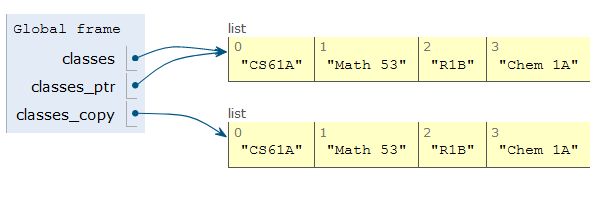
\includegraphics[scale=0.75]{pointers.PNG}
\end{center}
After a few weeks, you realize that you cannot keep up with the workload and you need to drop a class. You’ve chosen to drop Chem 1A. Based on what we know so far, to change our classes list, we would have to create a new list with all the same elements as the original list except for Chem 1A. But that is silly, since all we really need to do is remove the Chem 1A element from our list.

We can fix this issue with list mutation. In Python, some objects, such as lists and dictionaries, are mutable, meaning that their contents or state can be changed over the course of program execution. Other objects, such as numeric types, tuples, and strings are immutable, meaning they cannot be changed once they are created. Therefore, instead of creating a new list, we can just call classes.pop(), which removes the last element from the list.
\newpage
\begin{lstlisting}
>>> classes.pop() # pop returns whatever item it removed
"Chem 1A"
\end{lstlisting}

\begin{center}
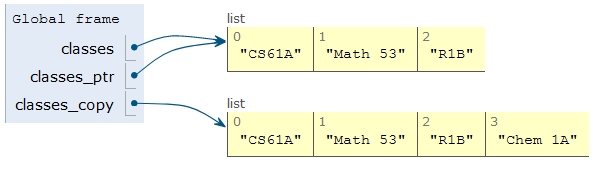
\includegraphics[scale=0.75]{pointers_mutate.PNG}
\end{center}

List methods that mutate:
\begin{itemize}
\item \lstinline{append(el)}: Adds el to the end of the list
\item \lstinline{extend(lst)}: Extends the list by concatenating it with lst
\item \lstinline{insert(i, el)}: Insert el at index i (does not replace element but adds a new one)
\item \lstinline{remove(el)}: Removes the first occurrence of el in list, otherwise errors
\item \lstinline{pop(i)}: Removes and returns the element at index i, if you do not include an index it pops the last element of the list
\end{itemize}
Ways to copy: list splicing ([start:end:step]), \lstinline{list(...)}


\begin{guide}
	\begin{blocksection}
	\textbf{Teaching Tips}
	\begin{itemize}
			\item Common Misconceptions:
			\begin{itemize}
				\item Students may be confused about the return value of mutation functions
				\begin{itemize}
					\item Try contrasting \lstinline{pop} with \lstinline{remove}, showing them how only \lstinline{pop} returns the element
					\item Tell them to reference the list mutability table
				\end{itemize}
			\end{itemize}
			\item The objectives for students are to:
			\begin{itemize}
				\item Distinguish between mutable and non-mutable objects
				\item The effects and return values of mutation functions
				\item Become comfortable with pointers and how to copy objects
			\end{itemize}
	\end{itemize}
	\end{blocksection}
\end{guide}
